\documentclass{standalone}
\usepackage[utf8]{inputenc}
\usepackage{tikz, pgfplots}

\pgfplotsset{compat=1.15}


\begin{document}
    
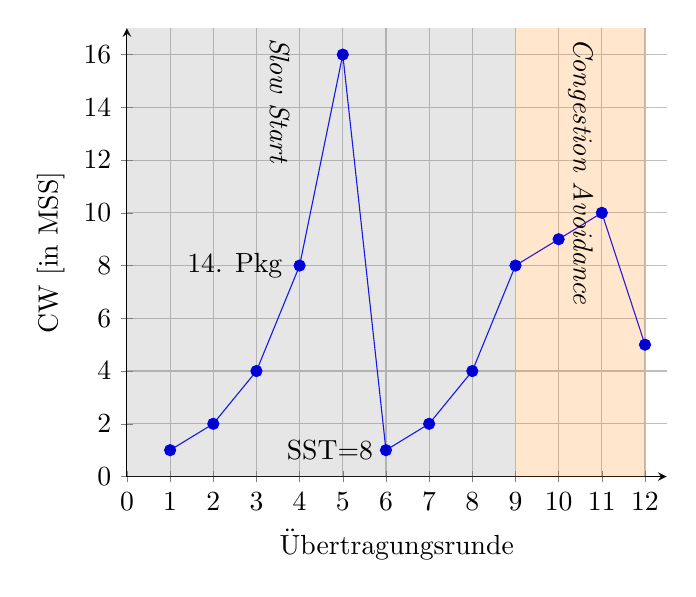
\begin{tikzpicture}
    \begin{axis}[
        axis y line = left,
        axis x line = bottom,
        xlabel      = {Übertragungsrunde},
        ylabel      = {CW [in MSS]},
        xtick       = {0,1,...,12},
        ytick       = {0,2,4,...,16},
        domain      = 0:12,
        xmin = 0, xmax = 12.5,
        ymin = 0, ymax = 17,
        grid = both,
      ]
      
    \addplot+[sharp plot] coordinates {
        (1,1) 
        (2,2)
        (3,4)
        (4,8)
        (5,16)
        (6,1)
        (7,2)
        (8,4)
        (9,8)
        (10,9)
        (11,10)
        (12,5)
    };

    \addplot[fill=gray,fill opacity=0.2,draw=none] coordinates {
        (9,17)
        (0,17)
        (0,0)
        (9,0)
    } node [right,pos=0.156,text=black,text opacity=1,rotate=-90] {\textit{Slow Start}};

    \addplot[fill=orange,fill opacity=0.2,draw=none] coordinates {
        (12,17)
        (9,17)
        (9,0)
        (12,0)
    } node [right,pos=0.065,text=black,text opacity=1,rotate=-90] {\textit{Congestion Avoidance}};

    \node at (axis cs:4.7,1) {SST=8};
    \node at (axis cs:2.5,8) {14. Pkg};

    \end{axis}
\end{tikzpicture}
\end{document}
